% !TEX encoding = UTF-8
% !TEX TS-program = pdflatex
% !TEX root = ../tesi.tex

%**************************************************************
\chapter{Progettazione}
\label{cap:progettazione}
%**************************************************************

In questo capitolo vengono spiegate in modo dettagliato le tecnologie utilizzate nella realizzazione del progetto, inoltre viene data una spiegazione generale di come è
stata progettata l'architettura generale del sistema e una più approfondita riguardante l'architettura del frontend, che era oggetto del progetto di stage.

%**************************************************************
\section{Tecnologie}

Di seguito viene data una panoramica delle tecnologie utilizzate.

\subsection*{Javascript}
\begin{figure}[H]
  \centering
  
\includegraphics[width=2cm]{immagini/logo-js.png}
  \caption{Logo Javascript}
\end{figure}
JavaScript è un linguaggio di programmazione orientato agli oggetti e agli eventi, comunemente utilizzato nella programmazione web lato client per la creazione di applicazioni web.
L'intera applicazione è stata scritta con questo linguaggio.

\subsection*{React}
\begin{figure}[H]
  \centering
  
\includegraphics[width=2cm]{immagini/logo-react.png}
  \caption{Logo React}
\end{figure}
React\footcite{site:react} è una libreria Javascript utilizzata per implementare \gls{UI}\glsfirstoccur lato frontend. React si basa sul concetto di component,
idealmente è una libreria che permette di costruire i propri component come fossere degli elementi \gls{HTML}\glsfirstoccur del \gls{DOM}\glsfirstoccur per poi poterli riusare nell'intera applicazione.

\subsection*{Redux \& Redux RTK}
\begin{figure}[H]
  \centering
  
\includegraphics[width=2cm]{immagini/logo-redux.png}
  \caption{Logo Redux}
\end{figure}
Redux\footcite{site:redux} è un contenitore dello \gls{stato}\glsfirstoccur per le applicazioni Javascript. Viene usato per la gestione centralizzata dello stato delle applicazioni sviluppate in React Javascript.
In particolare con la sua libreria Redux-Toolkit, permette una gestione dello stato semplice ed efficente.

\subsection*{MUI}
\begin{figure}[H]
  \centering
  
\includegraphics[width=2cm]{immagini/logo-MUI.png}
  \caption{Logo MUI}
\end{figure}
Material UI\footcite{site:mui} è una libreria React \gls{open-source}\glsfirstoccur che permette di implementare i Google's Material Design. Essa comprende una collezione di componenti React precostruiti che possono
essere facilmente adattati e messi in uso nella UI dell'applicazione.

\subsection*{React Router}
\begin{figure}[H]
  \centering
  
\includegraphics[width=2cm]{immagini/logo-recact-router.png}
  \caption{Logo React router}
\end{figure}
React Router è la libreria standard per il \gls{routing}\glsfirstoccur in React. Questa libreria permette la navigazione tra le varie viste dell'applicazione, permette di gestire le \gls{URL}\glsfirstoccur, e mantenere
la sincronizzazione tra URL e viste.
\newpage
%**************************************************************%
%**************************************************************%
%**************************************************************%
\section{Architettura dell'applicazione}
L'architettura generale dell'applicazione era già stata progettata prima dell'inizio dello stage in oggetto, e in parte già esistente. Il sistema si divide principalmente in tre parti:
\begin{itemize}
  \item \textbf{backend}
  \item \textbf{frontend}
  \item \textbf{object storage}
\end{itemize}

La comunicazione tra le diverse parti del sistema invece avviene con l'utilizzo di \textbf{\gls{API}\glsfirstoccur}.

\begin{figure}[H]
  \centering
  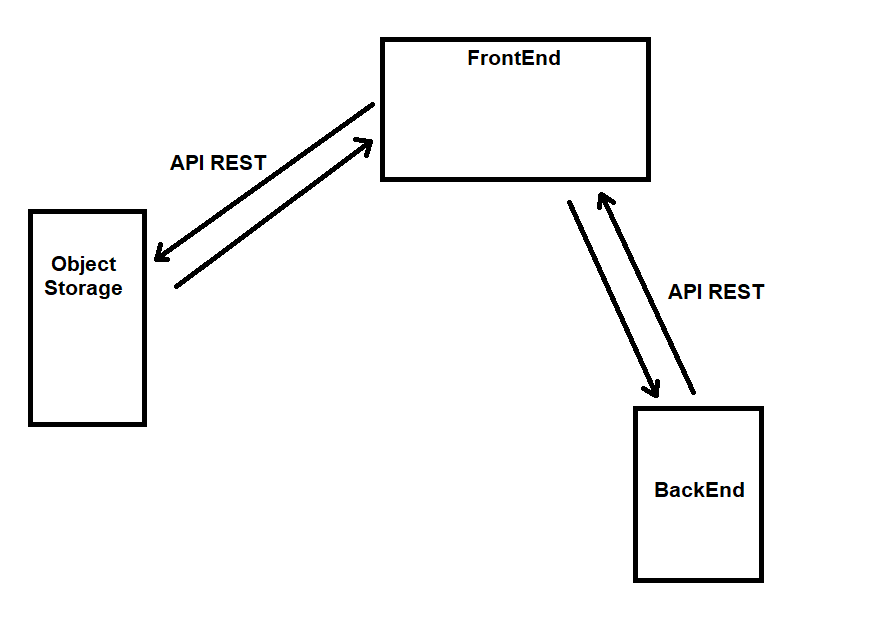
\includegraphics[width=\textwidth]{immagini/architettura-generale.png}
  \caption{Descrizione grafica dell'architettura generale dell'applicazione}
\end{figure}

%**************************************************************%
\subsection{Backend}
Il backend è un'applicazione a se stante realizzata interamente in Python, con architettura \gls{MVC}\glsfirstoccur. Questa architettura permette di separare completamente
la logica del prodotto dal modello dei dati, le viste non sono state approfondite in quanto lo scopo principale del backend è gestire e memorizzare i dati che vengono passati
dal frontend e non visualizzarli. Il backend espone delle particolari URL come \gls{endpoint}\glsfirstoccur per le chiamate \gls{REST}\glsfirstoccur del client frontend.
Il backend utilizza il modello (Model) per rappresentare i dati di interesse, il controller per gestirli, e la vista (View) per rappresentarli. Nel nostro caso, come già menzionato,
non dovendo rappresentare i dati (operazione che spetta al frontend), esso espone dell URL come endpoint per le chiamate REST proprio del frontend. In questo modo ogni volta che viene fatta
una richiesta su una corretta URL al backend, esso la interpreta con l'apposito controller, gestendo i dati strutturati come nel modello, e dopo aver completato la gestione
della richiesta, ne restituisce la risposta al frontend.

%**************************************************************%
\subsection{Frontend}
Il frontend dell'applicazione è generalmente la parte di interfaccia per l'utente, ossia quello che l'utente visualizza del nostro sistema e che gli da l'opportunità di interagire
con il backend. Nel nostro caso il frontend non fa solo da interfaccia utente ma gestisce anche dei dati nel proprio stato fin tanto che questi rimangono in \gls{sessione}\glsfirstoccur, in modo da
non fare continue richieste al backend che rallenterebbero molto il sistema a causa della mole dei dati da gestire e visto che non tutti i dati devono essere passati al backend.
Il frontend è stato scritto in JavaScript e in particolare usando il framework React, gestendo però lo stato esternamente usando Redux, questo porta ad un'architettura leggermente
più complessa dell'intero frontend ma da grandi benefici in quanto aiuta a mantenere per quanto possibile la separazione tra logica dell'applicazione e reppresentazione dei dati.
In generale l'architettura è quella della single page application, cioè una pagina che non necessita di essere totalmente ricaricata ad ogni modifica ma che va a modificare
soltanto la porzione interessata da uno specifico cambiamento.

%**************************************************************%
\subsection{Object storage}
L'object storage che si è deciso di utilizzare è minIO (scelta aziendale, legata anche ad altri progetti) e nel caso della nostra applicazione serve in particolare come stumento
per memorizzare i file con delle semplici richieste tramite API.
Questo ci permette essenzialmente due cose molto importanti, non doverci preoccupare troppo dei dettagli implementativi della memeorizzazione e allo stesso tempo poter
reperire agevolmente i file che ci servono. Per il caricamento di un file è necessario fare una richiesta PUT, ad una apposita URL di minIO passando come parametro il file che si desidera salvare.
Questa URL viene concordata tra backend e minIO stesso in modo da essere sempre univoca per ogni nuovo file caricato, questo comporta che l'operazione finale di salvataggio del file
comprenda tre richieste:
\begin{itemize}
  \item \textbf{frontend -> backend}: con questa richiesta il frontend comunica quale file vuole salvare al backend che può così memorizzarne i dati, in modo da tenerne traccia qualora si voglia in
        futuro reperire il file caricato;
  \item \textbf{backend -> minIO}: il backend richiede su un'apposita URL a minIO di comunicargli la vera e propria URL univoca sulla quale fare la richiesta di salvataggio del file,
        dopo che l'ha ottenuta la da in risposta al frontend;
  \item \textbf{frontend -> minIO}: il frontend dopo aver ricevuto la corretta URL sulla quale effettuare la richiesta PUT può eseguirla passando il file come parametro
\end{itemize}
Per la versione finale del progetto, non è escluso di rivedere questa parte che si prevede una delle più importanti, ma allo stesso tempo difficile da eseguire in modo efficace ed
efficiente. Per lo stato che il prodotto deve avere alla fine dello stage, invece, questa gestione è più che sufficiente.

%**************************************************************%
\subsection{API rest}
Le API rest sono il tramite tra le due applicazioni, backend e frontend, permettendo la comunicazione e il passaggio di dati. Vengono gestite nella parte frontend con Redux-tolkit,
uno strumento apposito per la gestione delle richieste API con Redux.
Le richieste del frontend interrogano il backend sugli appositi endpoint, e dopo aver ricevuto la risposta ne interpretano il risultato. Le richieste http rest possono essere di vario tipo,
ognuno dei quali rappresenta una particolare operazione che il client richiede al server di fare, nel nostro caso per la comunicazione tra backend e frontend sono state utilizzate richieste
di tipo GET e POST. Inoltre una particolare richiesta di tipo PUT viene effettuata dal frontend verso l'object storage minIO per l'upload dei file. Il linguaggio scelto per la comunicazione
tramite API è \gls{JSON}\glsfirstoccur, tra i più diffusi per questo tipo di operazioni per la sua semplicità di utilizzo.
\newpage
%**************************************************************%
%**************************************************************%
%**************************************************************%
\section{Architettura frontend}
L'architettura del frontend è stata progettata per essere poi implementata con le tecnologie che avevamo già in mente di usare e cioè in primis React e Redux. La progettazione del
frontend è molto semplice e si basa sull'interazione tra queste due tecnologie. React realizza tutte le nostre viste, tramite dei component che possono essere integrati tra loro
e riutilizzati, lo stato dell'applicazione invece è contenuto nello store di Redux, queste due entità comunicano in due modi:
\begin{itemize}
  \item \textbf{da component a store}: gli eventi Javascript/React che hanno bisogno di utilizzare lo stato dell'applicazione richiamano lo store con appositi metodi;
  \item \textbf{da store a component}: lo store invia ai component React le parti di stato che hanno richiesto o modificato così possono essere aggiornate;
\end{itemize}

Per capire nel dettaglio l'architettura del frontend ricorriamo al seguente schema di approfondimento.

\begin{figure}[H]
  \centering
  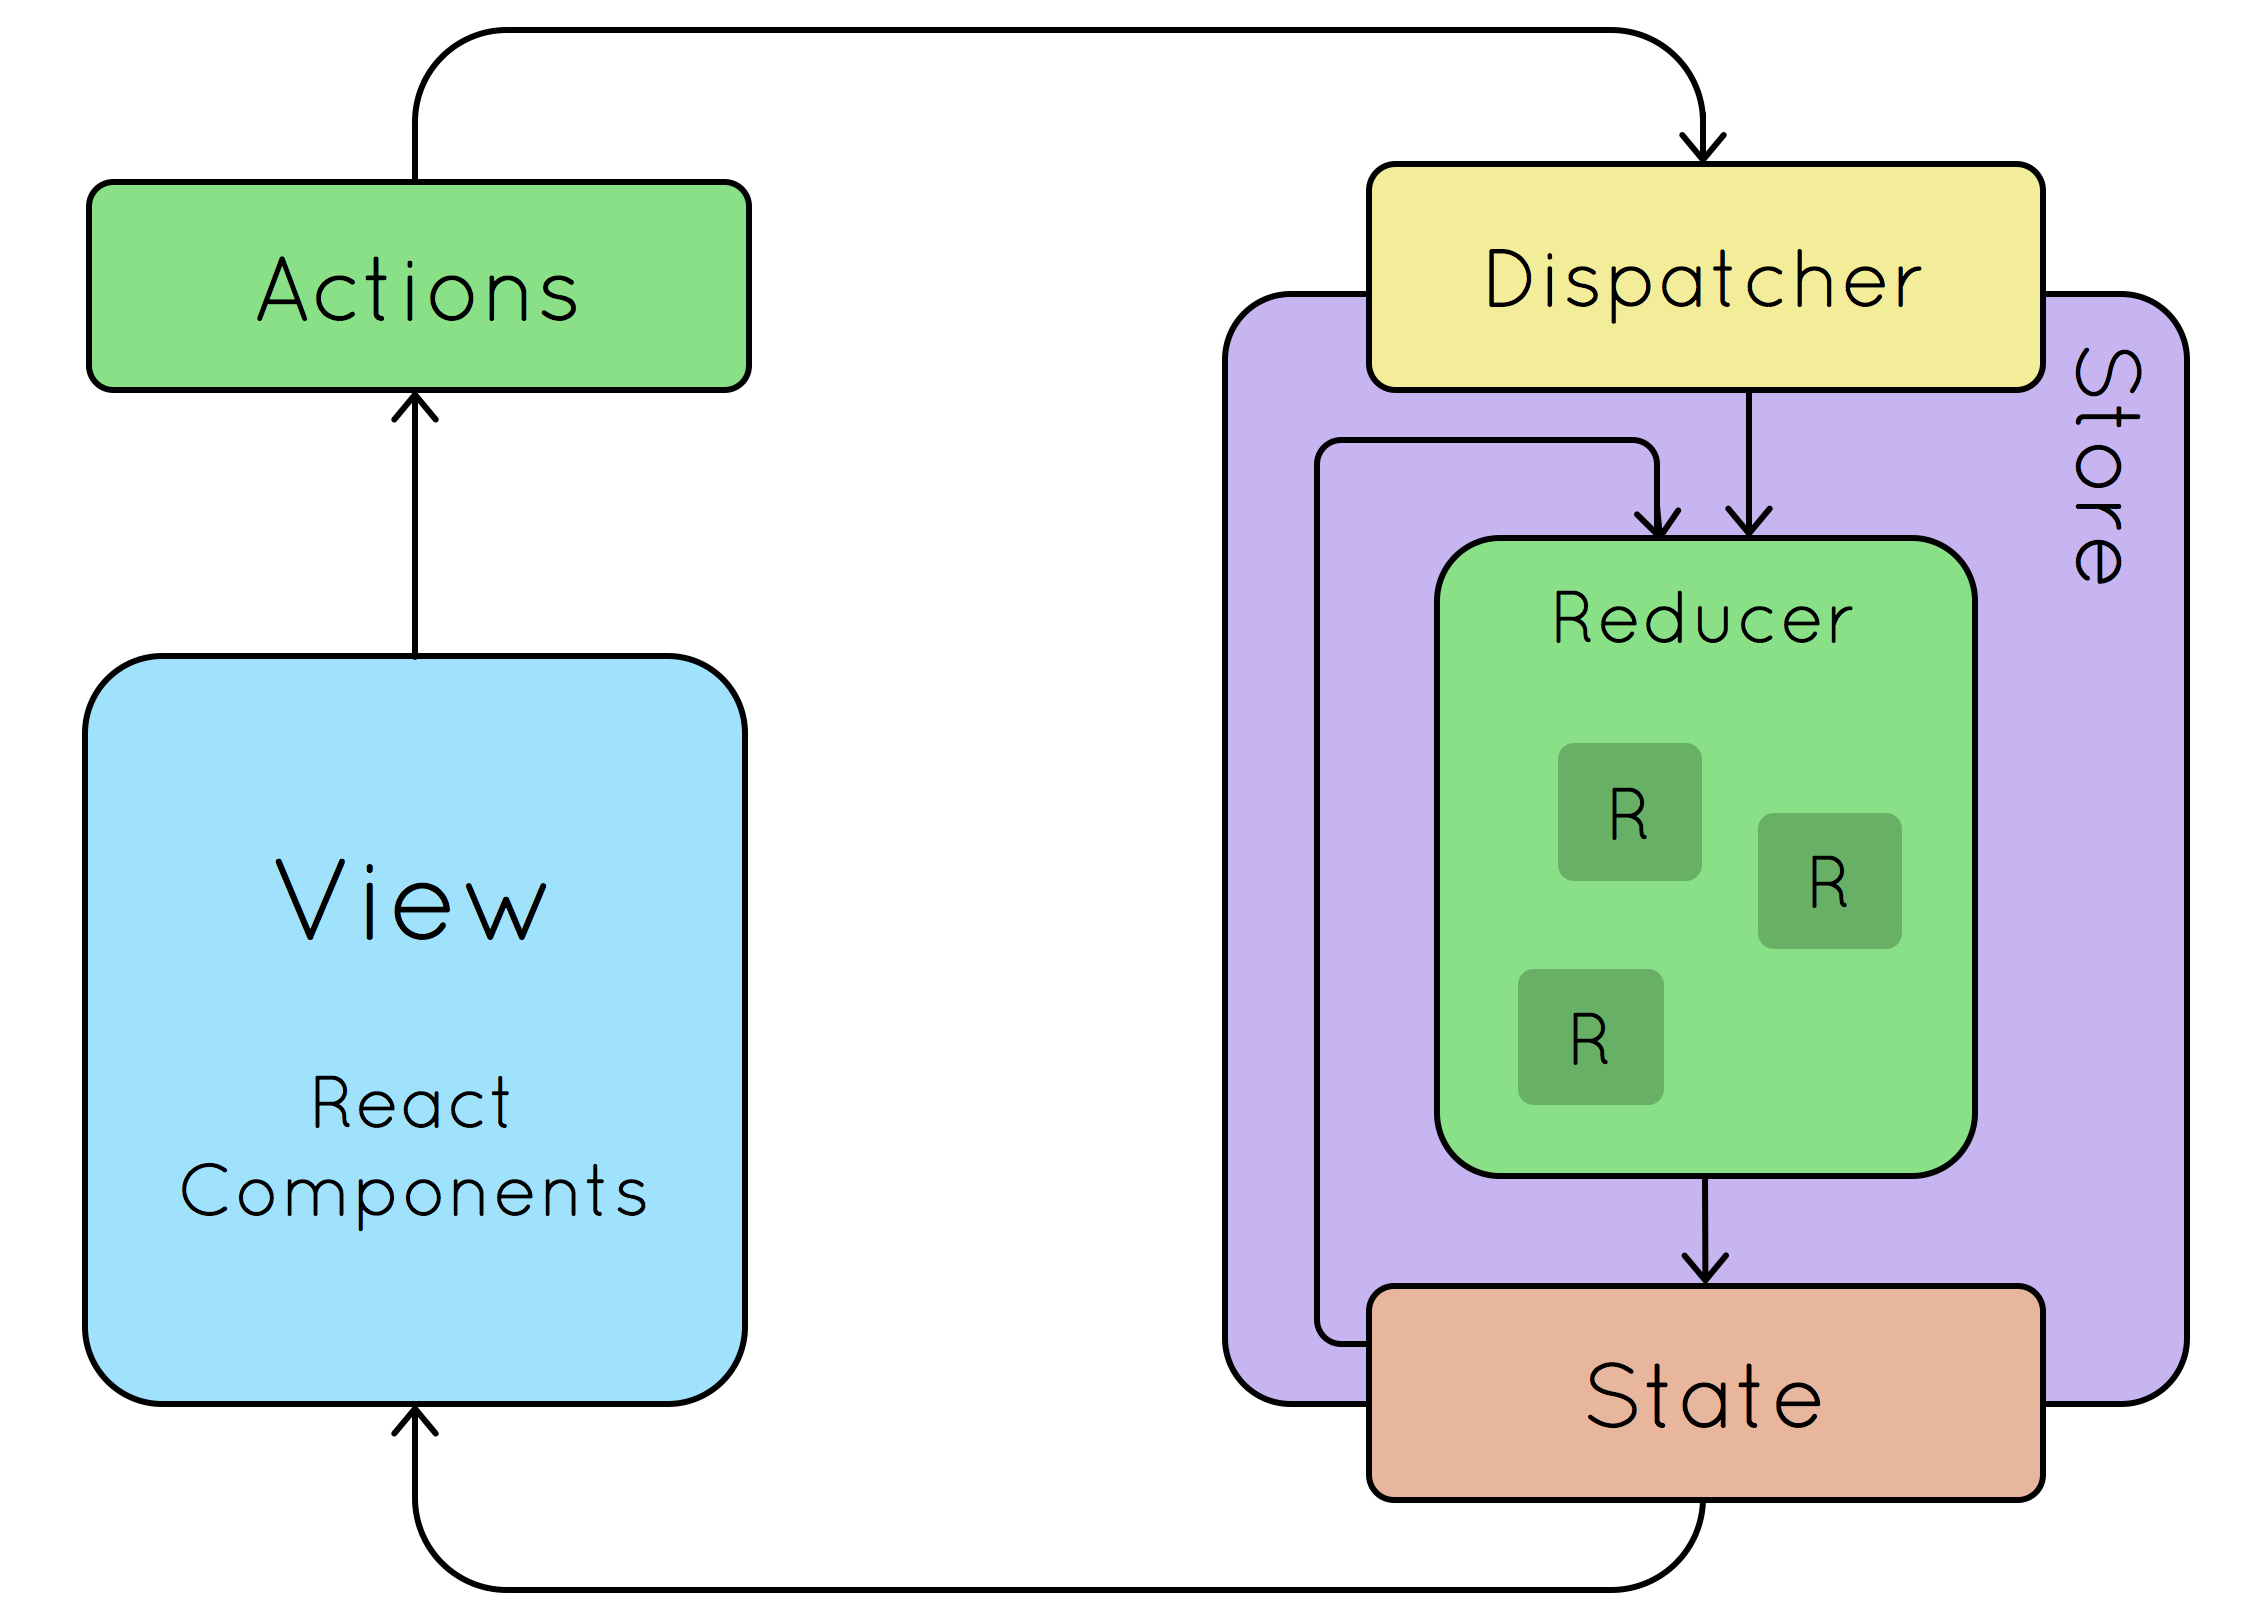
\includegraphics[width=\textwidth]{immagini/architettura-frontend.png}
  \caption{Descrizione grafica dell'architettura del frontend dell'applicazione}
\end{figure}

Il frontend dell'applicazione è stato progettato come una single page application, che mantiene completa seprarazione tra lo stato e la user interface, questo grazie proprio
all'utilizzo delle tecnologie scelte. Lo store Redux implementa quello che può essere visto come un modello di dati per i componenti React, essi invece svolgono sia la funzione
di vista che quella di controller, in quello che può essere idealizzato come un pattern \gls{MVVM}\glsfirstoccur, la natura delle tecnologie in causa però fa si che questo
pattern non sia stretto e vincolante per tutta l'applicazione. In generale l'applicazione risulta più semplicemente governata dal principio azione-reazione, infatti con la logica dei
component React risulta immediato associare ad ogni interazione dell'utente con la UI un evento. L'evento associato ad un azione dell'utente viene gestito in vari modi,
può coinvolgere una semplice modifica della UI, può implicare una modifica dello store e quindi una rielaborazione della UI (solo nelle parti coinvolte) oppure può lanciare una
richiesta tramite API al backend.
%   [[[esempio gestione eventi]]]
% UI -> event -> UI
% UI -> event -> store -> UI
% UI -> event -> API -> UI
% UI -> event -> API -> store -> UI
\newpage
%**************************************************************%
%**************************************************************%
%**************************************************************%
\section{Design Pattern utilizzati}
Alcuni design pattern utilizzati li abbiamo già citati, andiamo di seguito ad elencare quelli utilizzati dall'applicazione, alcuni sono nativi o intrisechi delle tecnologie utilizzate
altri invece pensati per la nostra specifica applicazione, l'utilizzo di tante tecnologie diverse integrate tra loro porta ad un utilizzo di alcuni design pattern in modo spurio,
questi quindi non sono presenti e implementati pedissequamente però risultano comunque in alcune forme o per alcuni aspetti chiave.
\begin{itemize}
  \item \textbf{MVVM}: come già citato in precedenza, l'integrazione tra React e Redux da vita ad una forma di questo pattern, se consideriamo lo store Redux come modello e i
        component React come viste con logica al proprio interno;
  \item \textbf{MVC}: non presente nel frontend ma bensi nel backend realizzzato in Python;
  \item \textbf{Observer}: nel frontend i componenti React sono dei subject sottoscritti allo stato dell'applicazione, quando questo cambia per qualsiasi motivo, i componenti
        vengono modificati
\end{itemize}

\newpage
%**************************************************************%
%**************************************************************%
%**************************************************************%
\section{Progettazione dell'applicazione}
Nel dettaglio della progettazione della nostra applicazione abbiamo pensato ad un funzionamento lineare, semplice ed intuitivo per l'utente finale, in modo da continuare a
perseguire le caratteristiche di velocità e facilità di utilizzo dell'applicazione, che ci eravamo prefissati in fase di analisi del progetto. L'architettura del sistema
permetterà il funzionamento che possiamo riassumere nei passi che spieghiamo di seguito.
\begin{figure}[H]
  \centering
  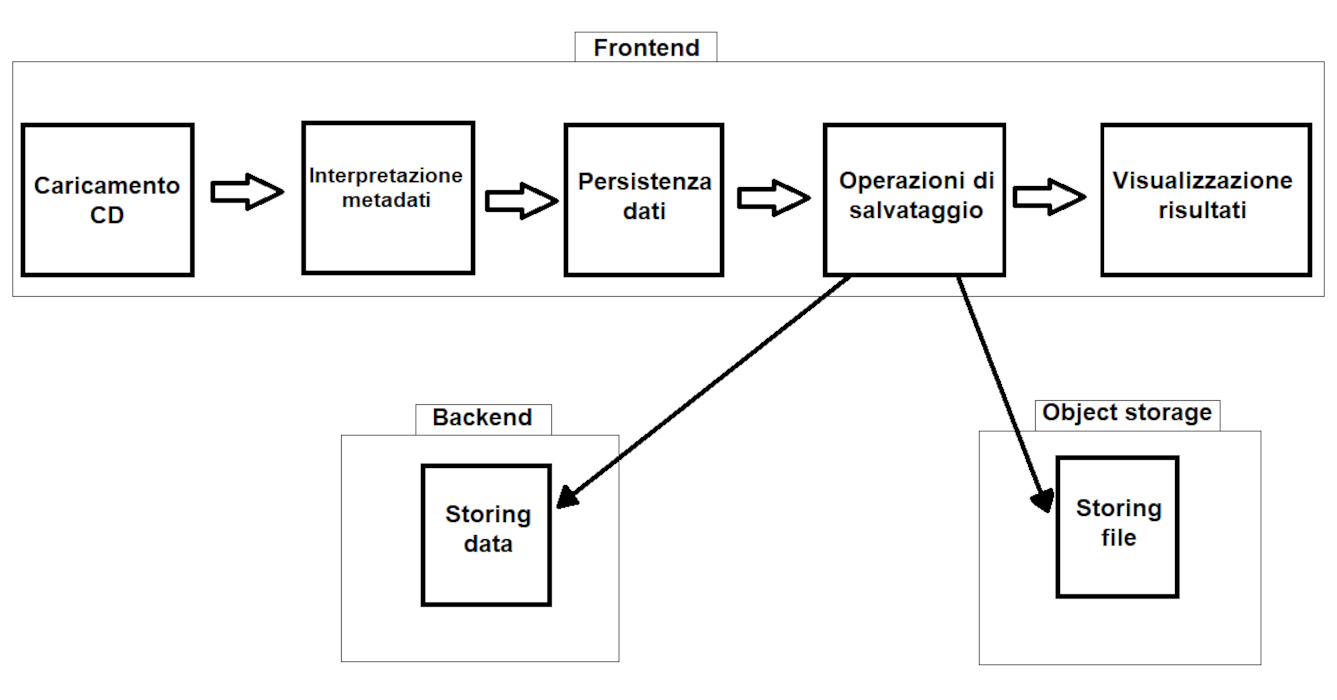
\includegraphics[width=\textwidth]{immagini/funzionamento.png}
  \caption{Schema del funzionamento della architettura per la nostra applicazione}
\end{figure}
\subsection*{Caricamento CD}
La prima operazione da fornire all'utente sarà il caricamento del CD contenete file audio e metadati che sono l'input della nostra applicazione.
\subsection*{Interpretazione metadati}
I metadati dovranno essere interpretati da una libreria di nostra creazione in modo da renderli disponibili all'interno dell'applicazione nei formati che possiamo trattare
agevolmente.
\subsection*{Persistenza dati/metadati sul frontend}
I metadati e i file caricati dall'utente e interpretati dalla nostra libreria ora sono pronti per essere memorizzati nel frontend, qui procederemo al trattamento di questi
dati con tutte le operazioni che metteremo a disposizione dell'utente, con lo scopo di creare i ticket che sono necessari.
\subsection*{Passaggio dati al backend}
Dopo che l'utente ha svolto tutte le operazioni sui dati che riteneva opportune, creando i ticket, i dati vengono passati al nostro backend per essere memorizzati
in modo permanente, contestualmente a questa operazione vengono trattate le traccie audio coinvolte nei ticket, come spieghiamo di seguito.
\subsection*{Storing file}
Nel momento in cui avviene la richiesta per il caricamento dei dati necessari alla creazione dei ticket verso il backend, una richiesta parallela verrà inviata all'object storage
per salvare i file audio coinvolti nella creazione di questi ticket. La risposta di queste due operazione positiva o negativa verrà data all'utente che nel caso una delle
due o entrambe non siano andate a buon fine potrà ripeterle.
\subsection*{Visualizzazione risultati frontend}
Per concludere, dopo che le operazioni di memorizzazione dei dati sul backend e salvataggio dei file sull'object storage sono andate a buon fine, questi dati con i relativi file
vengono inviati in risposta al frontend in modo che l'applicazione possa esporli all'utente, in una sorta di riepilogo dei dati coinvolti nell'operazione che è avvenuta con successo.


